\documentclass{article} \usepackage{maa-monthly}


\theoremstyle{theorem} \newtheorem*{theorem}{Theorem}

\theoremstyle{definition} \newtheorem*{definition}{Definition}
\newtheorem*{remark}{Remark}

\begin{document}

\title{A geometric proof of Darboux's theorem}

\author{Luqing Ye}

\maketitle

\begin{abstract}
By using Lagrange's mean value theorem and the intermediate value
theorem,we provide a geometric proof of Darboux's theorem.
\end{abstract}


\noindent
In this note we give a geometric proof of Darboux's theorem,with
the aid of Lagrange's mean value theorem and the intermediate value
theorem.After I completed the proof,I found that the proof is
essentially not new,Lars Olsen had already provided an extremely
similar proof in \cite{Lars}.However,I decide to publish my proof
because its geometric feature,and after all,there are slight
differences between our approach.

Darboux's theorem,which shows the intermediate property of
derivatives,can be stated as below.
\begin{theorem}[Darboux's theorem]
Let $I$ be an open interval.$a,b\in I$ and $a<b$.Let $f:I\to \mathbf{R}$ be a
differentiable function,and $f'(a)<f'(b)$.Then $\forall t\in
(f'(a),f'(b))$, there exists $\xi\in
(a,b)$,such that $f'(\xi)=t$.
\end{theorem}
\begin{figure}[h]\centering
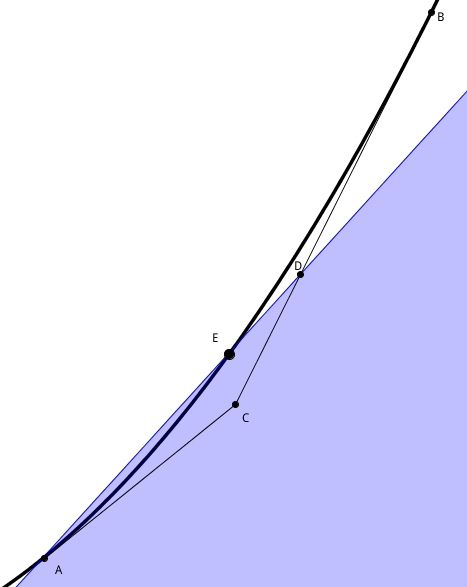
\includegraphics[width=0.5\textwidth]{A_geometric_proof_of_Darboux_theorem1.png}
  \caption{}
  \label{fig:1}
\end{figure}
\begin{proof}
  As shown in figure \eqref{fig:1},there are five points
  $A(a,f(a))$,$B(b,f(b))$,$C(x_c,y_c)$, $D(x_{d},y_{d})$,$E(x_e,y_e)$ in the figure.The curve represents the graph
  of the function $f$ over $(a,b)$.Line $AC$ is the tangent line of the curve at
  the point $A$.Line $BC$ is the tangent line of the curve at the
  point $B$. For an arbitrary point $D$ on the segment $BC$(excluding points
  $B,C$),line $AD$ must
  intersect with the curve at a point $E$ over the interval
  $(a,b)$.This is because,the slope of the line $AD$ is larger than
  the slope of the line $AC$(which is $f'(a)$),so the curve passing through the point
  $A$ must intersect with the shaded region(a closed half plane whose
  boundary is line $AD$) over the interval $(a,b)$,but this continuous curve also
  passes through the point $B$ which is not in the shaded region.So according to the intermediate value theorem,the curve must
  intersect with the line $AD$ at a point $E$ over the interval
  $(a,b)$.According to Lagrange's mean value theorem,there exists
  $\xi_1\in (a,x_e)$ such that 
\begin{equation}\label{eq:1}
f'(\xi_1)=\mbox{the slope of the line} ~AD.
\end{equation}

Similary,as shown in figure \eqref{fig:2},for an arbitrary point $D'$
on the segment $AC$(excluding points $A,C$),line $BD'$ must intersect with the curve at a
point $E'(x_e',y_e')$ over the interval $(a,b)$.This is because,the
slope of the line $BD'$ is smaller than the slope of the line
$BC$(which is $f'(b)$),so the curve passing through the point $B$ must
intersect with the shaded plane(a closed half plane whose boundary is
line $BD'$)over the interval $(a,b)$,but this continous curve also passes through
the point $A$ which is not in the shaded plane.So according to the intermediate value theorem,the curve must
  intersect with the line $BD'$ at a point $E'$ over the interval
  $(a,b)$.According to Lagrange's mean value theorem,there exists
  $\xi_2\in (x_e',b)$ such that
\begin{equation}\label{eq:2}
f'(\xi_2)=\mbox{the slope of the line}~BD'.
\end{equation}

Also,according to Lagrange's mean value theorem,there exists $\xi_3\in
(a,b)$ such that
\begin{equation}
  \label{eq:3}
  f'(\xi_3)=\mbox{the slope of the line}~AB.
\end{equation}

\begin{figure}[h]\centering
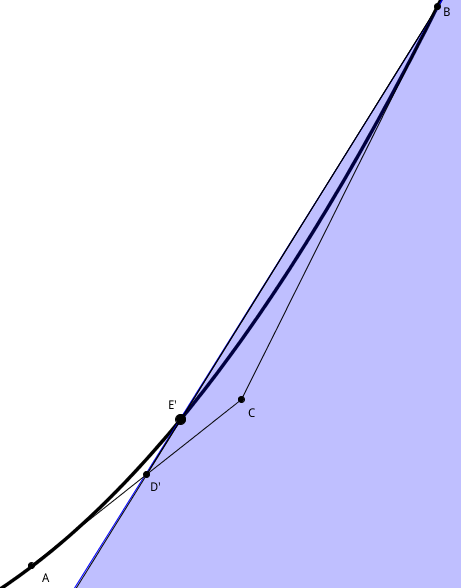
\includegraphics[width=0.5\textwidth]{A_geometric_proof_of_Darboux_theorem2.png}
  \caption{}
  \label{fig:2}
\end{figure}

It can be easily verified from elementary geometry that when $D$ and $D'$ move continuously over the segment $BC$ and $AC$
respectively,with the extreme points of both segments excluded,we have
\begin{align*}
&\{\mbox{the slope of the line}~AD\}\cup\{\mbox{the slope of the
  line}~BD'\}\cup\{\mbox{the slope of the line}~AB\}\\&=(\mbox{the slope of the line}~AC,\mbox{the slope of the line}~BC)=(f'(a),f'(b)).
\end{align*}

So Darboux's theorem is finally proved by combining this relationship with  equation \eqref{eq:1},
\eqref{eq:2} and \eqref{eq:3}.
\end{proof}
\begin{thebibliography}{1}
\bibitem{Lars} Lars Olsen , A New Proof of Darboux's Theorem ,\textit{Amer. Math. Monthly},\textbf{111} (2004)713--715.
\end{thebibliography}

\begin{biog}
\item[Luqing Ye] (yeluqingmathematics@gmail.com) is an undergraduate
  student at Hangzhou Normal University in Hangzhou,Zhejiang Province,China.
\end{biog}
\end{document}
